\section*{Условие}

В одной программе написать правила, позволяющие найти:
\begin{enumerate}
	\item Максимум из двух чисел;
 	\item Максимум из трех чисел.
\end{enumerate}
Для каждой программы реализовать два варианта: с использованием отсечения и без использования отсечения.  

Убедиться в правильности результатов.

\textbf{Для каждого случая пункта 2 обосновать необходимость всех условий тела.}

\textbf{Для одного} из вариантов \textbf{ВОПРОСА} и каждого варианта задания 2 \textbf{составить
таблицу}, отражающую конкретный порядок работы системы:

Т.к. резольвента хранится в виде стека, то состояние резольвенты требуется отображать
в столбик: (вершина – сверху). Новый шаг надо начинать с нового состояния резольвенты.  

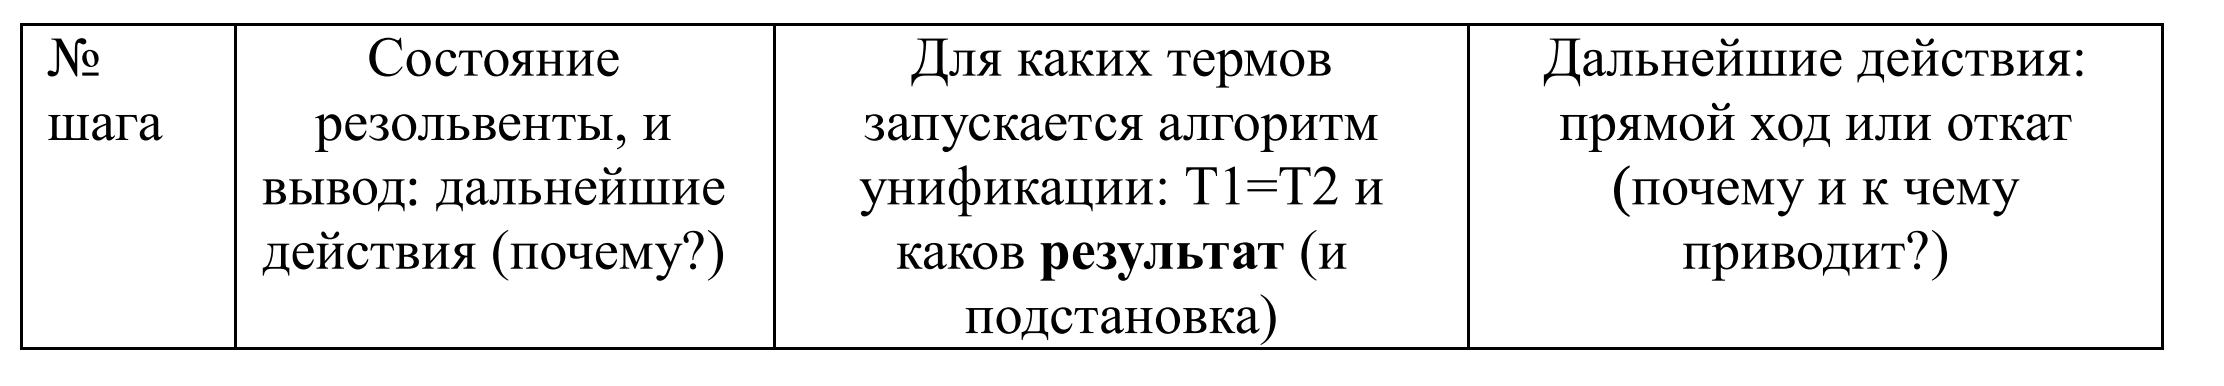
\includegraphics[scale=0.4]{./inc/img/tb_tmpl}

\section*{Решение}

\lstinputlisting[caption={Задание 1}, label={lst:t1}, language=lisp]{../src/main.pro}

В Таблицах \ref{tbl:1-1}-\ref{tbl:1-2} представлен порядок поиска ответа на вопросы 1 и 2.


\begin{landscape}
    \setlength{\LTcapwidth}{\linewidth}
    \begin{longtable}{|c|c|c|c|c|}
        \caption[Порядок формирования результата для 1-го вопроса]{Порядок формирования результата для 1-го вопроса} \label{tbl:1-1}\\
    
        \hline
            Шаг & Сравниваемые термы; & Дальнейшие & Резольвента & Подстановка \\
                & результаты & действия & & \\
        \endfirsthead
    
        \multicolumn{5}{l}
        {{\tablename\ \thetable{} -- продолжение}} \\
        \hline 
            Шаг & Сравниваемые термы; & Дальнейшие & Резольвента & Подстановка \\
                & результаты & действия & & \\\hline
        \endhead
        
        \endfoot
        \hline
        \endlastfoot
              & maxFromThree(22, 7, 11, R) & Прямой ход & maxFromThree(22, 7, 11, R) & \\
            1 & и maxFromTwo(A, B, A) & Переход к & &\\
			  & Главные функторы не равны & след. предл. & &\\
			\hline
			\dots & \dots & \dots & \dots & \dots \\
			\hline 
			5 & maxFromThree(22, 7, 11, R) и maxFromThree(A, B, C, A) & Прямой ход & 22 >= 7, 22 >= 11 & A = 22, B = 7, C = 11, R = 22\\
            \hline 
			6 & 22 >= 7 & Прямой ход & 22 >= 11  & A = 22, B = 7, C = 11, R = 22\\
            \hline 
			7 & 22 >= 11 & Нашли ответ & & A = 22, B = 7, C = 11, R = 22\\
            \hline 
			8 & maxFromThree(22, 7, 11, R) & Прямой ход & maxFromTwo(7, 11, Result) & B = 7\\
              & и maxFromThree(\_, B, C, Result) & & & C = 11 \\
            \hline 
			9 & maxFromTwo(7, 11, Result) & Прямой ход & A >= B & A = 7, B = 11\\
              & и maxFromTwo(A, B, A) & & & R = 11 \\
            \hline 
			10 & A >= B & Неудача, откат & & --- \\
			\hline
			\dots & \dots & \dots & \dots & \dots \\
			\hline
            30  & maxFromThree(22, 7, 11, R) & Завершение & maxFromThree(22, 7, 11, R) & \\
              & и maxFromThreeCut(\_, B, C, Result)& работы & &\\
              & Line, Sex) & 2 подст. & & \\
              & Главные функторы не равны & в рез-те & & \\
    \end{longtable}
\end{landscape}

\begin{landscape}
    \setlength{\LTcapwidth}{\linewidth}
    \begin{longtable}{|c|c|c|c|c|}
        \caption[Порядок формирования результата для 2-го вопроса]{Порядок формирования результата для 2-го вопроса} \label{tbl:1-2}\\
    
        \hline
            Шаг & Сравниваемые термы; & Дальнейшие & Резольвента & Подстановка \\
                & результаты & действия & & \\
        \endfirsthead
    
        \multicolumn{5}{l}
        {{\tablename\ \thetable{} -- продолжение}} \\
        \hline 
            Шаг & Сравниваемые термы; & Дальнейшие & Резольвента & Подстановка \\
                & результаты & действия & & \\\hline
        \endhead
        
        \endfoot
        \hline
        \endlastfoot
        
        \hline
              & maxFromThreeCut(22, 7, 11, R) & Прямой ход & maxFromThreeCut(22, 7, 11, R) & \\
            1 & и maxFromTwoCut(A, B, A) & Переход к & &\\
			  & Главные функторы не равны & след. предл. & &\\
			\hline
			\dots & \dots & \dots & \dots & \dots \\
			\hline 
			7 & maxFromThreeCut(22, 7, 11, R) & Прямой ход & 22 >= 7, 22 >= 11, ! & A = 22, B = 7\\
			& и maxFromThreeCut(A, B, C, A) & & & C = 11, R = 22\\
            \hline 
			8 & 22 >= 7 & Прямой ход & 22 >= 7, ! & A = 22, B = 7, C = 11, R = 22\\
            \hline 
			9 & 22 >= 11 & Нашли ответ & ! & A = 22, B = 7, C = 11, R = 22\\
			\hline 
			10 & ! & Завершение & & A = 22, B = 7, C = 11, R = 22\\
			   & & работы & &\\
               & & 1 подст. & & \\
               & & в рез-те & & \\
    \end{longtable}
\end{landscape}
\section*{Контрольные вопросы}

\subsection*{Какое первое состояние резольвенты?}

Заданный вопрос (goal в коде программы).

\subsection*{В каком случае система запускает алгоритм унификации?}

Система запускает алгоритм унификации автоматически при необходимости доказать что-то.

\subsection*{Каково назначение и результат использования алгоритма унификации?}

Унификация – логический вывод. Результат – подстановка.

\subsection*{В каких пределах программы переменные уникальны?}

Именованная переменная уникальна в предложении, в котором она используется. Анонимные переменные всегда уникальны.

\subsection*{Как применяется подстановка, полученная с помощью алгоритма унификации?}

Подстановка применяется к целям в резольвенте путем замены текущей переменной на соответствующий терм.

\subsection*{Как изменяется резольвента?}

Преобразования резольвенты выполняются с помощью редукции. Редукцией цели G с помощью программы P называется замена цели G телом того правила из P, заголовок которого унифицируется с целью. Новая резольвента образуется в два этапа:
\begin{itemize}
    \item в текущей резольвенте выбирается одна из подцелей и для неё выполняется редукция;
    \item к полученной конъюнкции целей применяется подстановка, полученная как наибольший общий унификатор цели и заголовка сопоставленного с ней правила.
\end{itemize}

\subsection*{В каких случаях запускается механизм отката?}

Механизм отката запустится в случае неудачи алгоритма унификации.